

\documentclass[10pt]{beamer}

%\usepackage{pgfpages}
%\mode<handout>{\setbeamercolor{background canvas}{bg=black!20}}
%\pgfpagesuselayout{4 on 1}[letterpaper,border shrink=5mm]

\usepackage{xcolor}
\usepackage[utf8]{inputenc}
\usepackage{amsmath, amsfonts}
\beamertemplatenavigationsymbolsempty
\setbeamertemplate{footline}[frame number]

\definecolor{dgreen}{rgb}{0.,0.6,0.}
\definecolor{highlight}{rgb}{0.,0.6,0.}

\usepackage{multimedia}

\begin{document}

\title{Cancer classification based on miRNA profiles using ASP} 
\author{K.Becker and H. Klarner}
\date{Berlin, Mai 2016}

\institute{
Freie Universität Berlin, Germany
}

% logo of my university
\titlegraphic{\vfill
\includegraphics[width=2cm]{FU-Logo}\hspace*{4.75cm}~%
   
\includegraphics[width=2cm]{BMBF-Logo}
}

\frame{\titlepage}


%{\tiny R. Thomas. "Regulatory networks seen as asynchronous automata." JTB, 1991}



\begin{frame}{Selective cell targeting}
\begin{center}
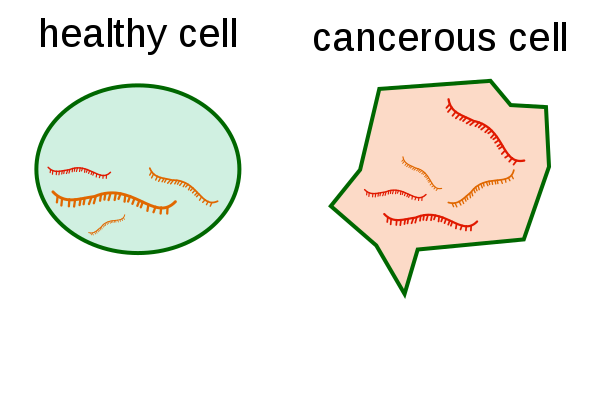
\includegraphics[scale=0.3]{cells.png}
\end{center}
\end{frame}



\end{document}

 
\begin{frame}{Boolsche Netzwerke}{Fixpunkte}
 \begin{center}\includegraphics[width=.7\linewidth]{../images/boolean_networks_fixpunkte}\end{center}
 \begin{itemize}
  \item Lösung: $x=101$
 \end{itemize}
 
\end{frame}
